\documentclass[10pt,conference,compsocconf]{IEEEtran}

\usepackage{hyperref}
\usepackage{graphicx}	% For figure environment


\begin{document}
\title{Machine Learning - Project 1}

\author{
  Alessandro Arrigoni, Emiljano Gjiriti, Paul M\"unnich\\
  \textit{Department of Computer Science, EPFL, Switzerland}
}

\maketitle

\begin{abstract}
 The detection of the Higgs boson particle is a classical machine learning task. As the particle decays very fast, not the particle itself is observed but the signature of its decay. Many decay signatures look very similar and it is up to machine learning models to determine whether the signal is a result of the Higgs boson or another process or particle in the background. In this study, a regression model with a high accuracy to determine the presence of Higgs boson is developed. 
 
 short description of obtained model (specifications+accuracy).

\end{abstract}

\section{Introduction}

In the first machine learning project, the methods learned in the course are applied in the context of the Higgs boson detection problem.
The data provided by CERN consists of thirty different features registered. In a first step, the data is preprocessed and analyzed to obtain the significant information from the input.
Afterwards, different techniques to determine regression models are applied and the most successful is identified using cross validation. 

\section{Data Analysis and Feature Engineering}
\label{sec:Data Analysis}

The raw training data provided by CERN consists of thirty features and a corresponding indication, whether the decay of Higgs boson was observed. Some data were not or could not be measured and hence are indicated by the value -999. In a first step, the given data is cleaned from these unmeasured values. The unmeasured values are set to 0 and afterwards replaced by the average value of the corresponding column. In the next step, the input data is standardized. 

To identify insignificant features, thirty plots - one for each feature - plot the result \textit{y} over each feature. variables that result in a constant value for the range of the variable are considered insignificant and hence can be removed from the input data.

In the next step, redundant information is removed from the input data. A plot for every feature against every other feature unveils pairwise correlations between two features. For an easier evaluation of these correlations, the corresponding correlation coefficient is calculated for each pair of features and visualized as shown in figure (...). Based on this analysis, columns 5, 9, 12, 21, 22, 23, 29 are left out due to a high correlation with the remaining features.


\section{Fitting a linear model}
\label{sec:fitting}

The approach applies the linear regression with the mean squared error (MSE) cost function. The linear regression is implemented in three different ways: The first one applies the normal equations, the second one applies gradient descent (GD) and the third one apples stochastic gradient descent (SGD) 




%\subsection{Figures and Tables}
%
%\begin{figure}[tbp]
%  \centering
%  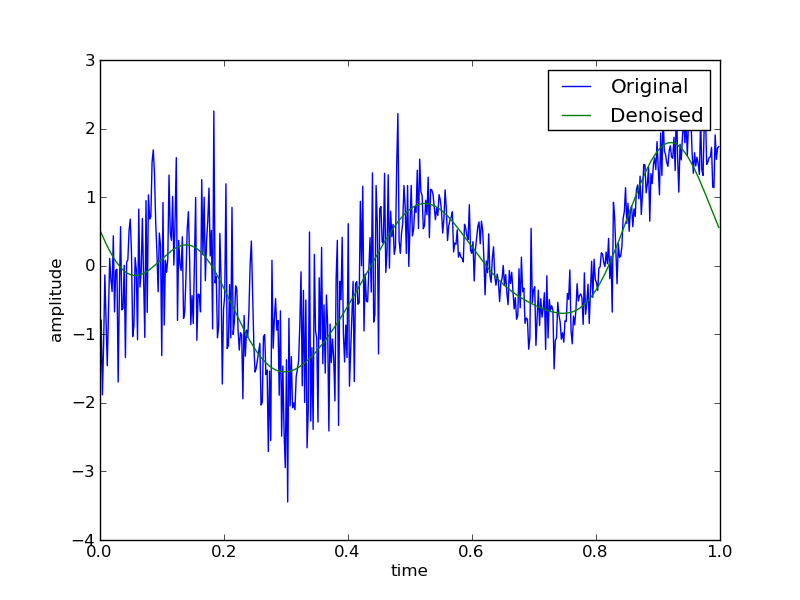
\includegraphics[width=\columnwidth]{denoised_signal_1d}
%  \caption{Signal compression and denoising using the Fourier basis.}
%  \vspace{-3mm}
%  \label{fig:denoise-fourier}
%\end{figure}
%\begin{figure}[htbp]
%  \centering
%  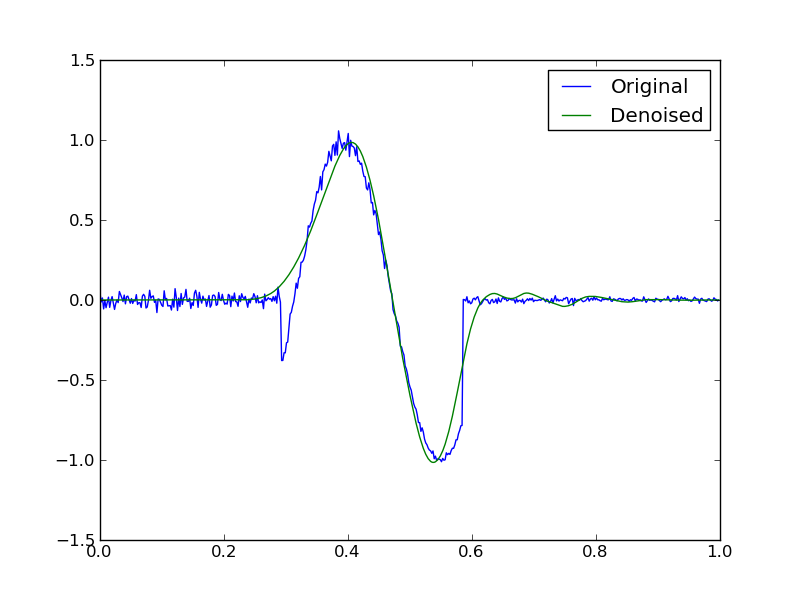
\includegraphics[width=\columnwidth]{local_wdenoised_1d}
%  \vspace{-3mm}
%  \caption{Signal compression and denoising using the Daubechies wavelet basis.}
%  \label{fig:denoise-wavelet}
%\end{figure}


%\begin{table*}[htbp]
%  \centering
%  \begin{tabular}[c]{|l||l|l|l|}
%    \hline
%    Basis&Support&Suitable signals&Unsuitable signals\\
%    \hline
%    Fourier&global&sine like&localized\\
%    wavelet&local&localized&sine like\\
%    \hline
%  \end{tabular}
%  \caption{Characteristics of Fourier and wavelet basis.}
%  \label{tab:fourier-wavelet}
%\end{table*}

\
%\subsubsection{Equations}
%
%There are three types of equations available: inline equations, for
%example $y=mx + c$, which appear in the text, unnumbered equations
%$$y=mx + c,$$
%which are presented on a line on its own, and numbered equations
%\begin{equation}
%  \label{eq:linear}
%  y = mx + c
%\end{equation}
%which you can refer to at a later point (Equation~(\ref{eq:linear})).

%\subsubsection{Tables and Figures}
%
%Tables and figures are ``floating'' objects, which means that the text
%can flow around it.
%Note
%that \texttt{figure*} and \texttt{table*} cause the corresponding
%figure or table to span both columns.





\bibliographystyle{IEEEtran}
\bibliography{literature}

\end{document}
